\documentclass[12pt,a4paper]{uwthesis17}

% Original customization work for UoW by Stephen Joe, et al. of the Maths Department
% Tweaked for ENGEN582 reports by David Bainbridge, et al. of the Computer Science Department 

% For a useful resource on other possible customisations, see:
%   https://codeinthehole.com/guides/writing-a-thesis-in-latex/

\usepackage[utf8]{inputenc}
\usepackage[T1]{fontenc}

% Times font used for both text and mathematical chars
\usepackage{mathptmx}

\usepackage{amsmath, amssymb, amsthm, amsxtra}
\usepackage{graphicx,color}
\usepackage{subfigure}
\usepackage{enumitem}
\usepackage[perpage]{footmisc}
\usepackage{listings}
\usepackage{caption}
\usepackage{float}
\usepackage{tabularx}
\usepackage{needspace}
\usepackage{ltablex} % Allows for multi-page tables with automatic width adjustment

\keepXColumns

\usepackage[
backend=biber,
style=ieee,
sorting=none,
mincitenames=1,
maxcitenames=1,
url=false,
eprint=false,
doi=false,
isbn=false
]{biblatex}
\addbibresource{references.bib}
\AtEveryBibitem{\clearlist{language}}
\AtEveryBibitem{\clearfield{note}}

\lstset{basicstyle=\ttfamily}

\usepackage[left=2.0cm, right=2.0cm, top=2.0cm, bottom=2.0cm, includefoot]{geometry}
% If interested in using 'fancyhdr' add in to the above:
% headheight=13.6pt

% Save the original tabularx definition
\let\origtabularx\tabularx

% Redefine tabularx to include \needspace before the table
\renewcommand{\tabularx}[2]{%
    \vspace{0.4cm}
    \needspace{2\baselineskip} % Adjust this based on your requirements
    \origtabularx{#1}{#2} % Call the original tabularx with the same arguments
}

\def\degree{Bachelor of Engineering (Hons)}
\def\thesis{R\&D report (Dissertation)}

\renewcommand{\figurename}{Fig.}


\title{Integration of cloud computing paradigms for performant analysis of simulated process engineering applications}

\author{
  Caleb Archer \\
  Supervised by: \\
  Mark Apperley, Tim Walmsley
}

\begin{document}

\pagenumbering{roman}

\maketitle

\setcounter{page}{2}

\begin{abstract}

\end{abstract}

\begin{acknowledgements}

\end{acknowledgements}

\begin{authorship-declaration}

\end{authorship-declaration}

\tableofcontents

\listoffigures

\listoftables

\newpage

\pagenumbering{arabic}
\setcounter{page}{1}

\section{Project aim}

The process systems engineering (PSE) field is critical to enabling detailed analysis and optimisation of industrial chemical processes. Despite this, modernisation of accessible optimisation software tools and techniques has slowed, with most software-based analysis performed via desktop applications constrained by the resource limits of local systems. More efficient optimisation techniques are available, but require software programming proficiency not held by the common process engineer. The cloud computing sector has significantly advanced the ability to run and deliver software in a distributed fashion, without requiring clients to procure and maintain physical hardware. Cloud-native software systems are better positioned to respond to dynamic usage and allocate computational resources efficiently based on need. There has been minimal convergence of the PSE and cloud computing fields.

This work details and evaluates the development of a cloud-native PSE software platform (the Ahuora Digital Platform) on a physical Kubernetes cluster, comparing the performance of the different software components running on the cluster versus a local deployment of said components.

% Is it worth stating some new research questions? I didn't actually create new research questions at the end of the literature review lol
\section{Background}

\section{Summary of literature review}

\chapter{Project Alignment within Collaborative Work}

\section{Kubernetes cluster architecture}

\section{Performance analysis experiment components}
\subsection{Controlled environment}

Difficulties were encountered obtaining consistent results when conducting ad hoc performance analysis experiments. Because of the usage of a 4G router for providing internet access to the Raspberry Pi cluster, highly variable bandwidth and latency conditions were encountered. One performance test with increasing load up to sixty requests per second might encounter exponentially increasing response times half-way during the test, while another repetition would see this occur three-quarters through the test. 

Another problem caused by relying on 4G mobile network infrastructure is the upper bandwidth limitation. The 4G router in use has (in its physical position in a lab) a peak download speed of \textasciitilde50.0 Mbit/second (\textasciitilde6.25 Mbyte/second), and an upload speed of \textasciitilde20.0 Mbit/second (\textasciitilde2.5 Mbyte/second). With increasing request rates during performance tests, a bandwidth bottleneck can be encountered, with the cluster unable to serve data because of a lack of sufficient capacity. Though perfect bandwidth and latency stability cannot be expected on the internet, mobile networks are especially prone to instability, and inhibit the ability to replicate a standard environment for applications deployed to ``the cloud'', i.e. a datacentre with high bandwidth capacity. This is exarcerbated by the usage of Cloudflare Tunnel on the cluster to enable external access, which provides a lower bound on maximum bandwidth than if the router was directly accessible via the internet.

To conduct consistent load-tests that provide a higher signal to noise ratio, a stable cloud infrastructure environment was simulated. Load-tests were performed from the ingress node, sending requests to the Kubernetes control node over the LAN (local area network) provided by the network switch. An Auckland-based data centre environment will be replicated, with an expected latency of 5 miiliseconds from an in-country client device to the data centre. This latency will be simulated via the \verb|tc| Linux command as depicted in Listings \ref{lst:pre-test-latency} and \ref{lst:post-test-latency}. The \verb|tc| command allows the traffic travelling via a particular network interface to have artificial constraints added, such as with bandwidth and latency. Prior to every test, 5 milliseconds of latency was added, and then removed after each test.

\begin{center}
    \begin{minipage}{\linewidth}
    \centering
    \begin{lstlisting}[language=bash, caption={Pre-test latency simulation command},label=lst:pre-test-latency]
    
    sudo tc qdisc add dev eth0 root netem delay 5ms
    
    \end{lstlisting}
    \end{minipage}
\end{center}

\begin{center}
    \begin{minipage}{\linewidth}
    \centering
    \begin{lstlisting}[language=bash, caption={Post-test latency simulation teardown},label=lst:post-test-latency]
    
        sudo tc qdisc del dev eth0 root netem
    
    \end{lstlisting}
    \end{minipage}
\end{center}

% ^^ fix stupid centreing and spacing later ^^

% Collect data to demonstrate the instability of external access %

% Show maximum LAN bandwidth results

% Show results of added latency perhaps.

\subsection{Controlling variables}

As with any valid experiment, any one load-test carried out assesses the performance differences observed after modifying one variable. For example, the number of replicas for a Kubernetes deployment, in one set of experiments, have been varied, while all other configuration fields have been kept the same. In some experiments, an entire block of configuration (such as the presence of a \verb|HorizontalPodAutoscaler| in a \verb|Deployment|) have been independently assessed, and everything else controlled. 

\subsection{Preliminary performance modelling}
\subsection{Empirical comparison}
\subsubsection{Grafana k6 load-testing}

Grafana k6\footnote{Grafana k6: https://k6.io/}, or k6, is a load-testing tool for assessing the performance of local and remote software systems. It is a script-based tool, where developers use JavaScript to define their testing logic, scenarios, and metrics, and then these tests are run using a Go-based custom JavaScript runtime to minimise test performance overheads.

k6 tests are built around the concept of a ``Virtual User'' or VU, which represents one unit of work that carries out one iteration of the defined test logic. The test logic may carry out a simple action such as making a request to a website at some URL, and waiting for the response. During a test, k6 displays the number of iterations being completed by VUs, as well as the number of VUs that are stalled in waiting for their respective request responses. VUs are run concurrently within a runtime thread pool, with each VU requiring an allocation of memory depending on the work each test iteration does.

Test scenarios can be defined in a number of ways. One test may utilise a ``constant arrival rate'' executor, which attempts to send a fixed number of test iterations for every unit of time (seconds, minutes, etc.) using the available pool of VUs. Another could use a ``ramping arrival rate'' executor, which can be configured to start an increasing, decreasing, or even constant number of test iterations per unit of time, at different stages of the test.

There are several other scenario executors that can be used within k6, but these have the possibility of skewing test results. For example, the ``constant VUs'' executor tries to use a set number of VUs to launch as ``as many iterations as possible''. However, if the executor detects that the time required to complete an iteration increases beyond a certain limit (i.e. the request response time is increasing), it will decrease the iteration start rate, and thereby reduce the number of requests being started. When the goal is to test how a system responds under specific conditions, this style of execution is unfavourable, given that it will dynamically change the test conditions. As such, the executors utilised in testing the Ahuora Digital Platform have been limited to the constant and ramping arrival rate exectors.

\subsubsection{Active test client and system monitoring}

As performance tests were carried out, the Grafana monitoring tool was used to gain insight into how the tests were impacting the different parts of the cluster, including at the container level, node level, and the overall cluster. Apart from this, it was important to ensure that the intended loads could actually be generated by the client sending the requests to the system. If the client encounters CPU or memory limits when attempting to generate load, then test results will be affected by the performance of the client, rather than the system, and prevent any meaningful insights being obtained. To ensure that client-side test throttling is not taking place, the \verb|htop| Linux command was used to observe client CPU and memory usage. The thresholds of 90\% CPU usage (across all cores) and 80\% memory usage were chosen as causes for concern for test validity.

\subsection{Key metrics}
\subsubsection{Response time}
\subsubsection{Throughput}
\subsubsection{Quantile comparison}
\subsubsection{Error rate}
\subsection{Secondary metrics}
\subsubsection{CPU usage}
\subsubsection{Memory usage}

\section{Performance analysis experiments}
\subsection{Benchmark environment}

A reference point to compare collected test metrics against is needed to obatin meaningful insights with respect to performance improvements. A series of benchmarks were created to compare various Kubernetes cluster configuration impacts against. As one of the purposes of this project is to analyse how transitioning to a cloud-based system can affect the performance of a process engineering simulation application, all benchmarks assess this system running entirely on one system, with all interprocess communication taking place locally.

This local deployment is set up with Docker Compose\footnote{Docker Compose: https://docs.docker.com/compose/}, which allows a set of containerised software components to be configured and run with ease on a local system. Docker configures a private network shared by each container defined in the configuration manifest, and enables DNS-based communication between containers. The manifest used in benchmarks defines four containers: the Django API server, a PostgreSQL database, the PgBouncer database connection pooler, and the IDAES mathematical solver service. The API server uses PgBouncer as its database endpoint, which manages the reuse of connections made to the database. 

\subsection{Test scenarios}

Various load profiles are used to assess system performance and dynamics. This allows for observation of whether the system is appropriately tuned or capable of responding to both flat and variable load profiles, as well as handling extended load periods. Two core API endpoints available on the Django API server are used for each test scenario, as described in Table \ref{table:test-api-endpoints}. Software versions used are: Django API 0.0.17, IDAES worker 0.0.10 and Postgres 16.4.

\begin{table}[h]
    \centering
    \begin{tabularx}{\textwidth}{|p{0.2\textwidth}|X|p{0.28\textwidth}|}
        \hline
        \textbf{Test type} & \textbf{Endpoint} & \textbf{Description} \\ \hline
        Unit operation retrieval (UOR) & /api/unitops/unitops/?flowsheetOwner=\{id\} & Retrieves all unit operations belonging to a particular flowsheet. \\ \hline

        Flowsheet solving (FS) & /api/solve/idaes/ & Serialises a flowsheet and sends an internal request to the IDAES service to solve the flowsheet's parameters. \\ \hline
    \end{tabularx}
    \caption{API endpoints used for system testing}
    \label{table:test-api-endpoints}
\end{table}

The unit operation retrieval endpoint interacts with the Django API server and the PostgreSQL database. The flowsheet solving endpoint interacts with both of these, as well as the IDAES service. The specific load profiles used against either endpoint will differ, as these endpoints have dissimilar baseline response times. The time required to make a single unit operation retrieval request is between 20 and 40 milliseconds, while a solve request may take 500 to 1000 milliseconds.

% Perhaps get a smoke test done at 1 request per second for both endpoints.

Flat load profiles will have initial ramp-up and ramp-down periods between their core profiles to provide corresponding system warm-up and cooldown periods. These periods will be short, fixed at 5\% of the total test duration each.

To avoid individual tests skewing the overall results, each test scenario will be run three times, with the resulting data averaged across the three trials.

\subsubsection{Pre-trial scenario set up}

Though these experiments do not interact with nor test the Ahuora Digital Platform's user interface, a React-based front-end, it is still necessary to construct a solvable flowsheet that can be used to retrieve unit operations from, and make solve requests. This flowsheet needs to be consistent between test scenarios and their trials. At the same time, the flowsheet needs to be deleted after usage during a trial to avoid an excessive and duplicated presence for users of the live platform when viewing available flowsheets. As such, it was necessary to construct pre and post-trial flowsheet set up and teardown scripts.

These Node.js-based scripts use the existing Django API to create (and delete) a flowsheet, unit operation, and all their corresponding properties and elements of configuration. The flowsheet constructed consists of a single pump with two material streams, one serving as input to the pump, and another as output. The specific steps involved in creating the flowsheet are:

\begin{enumerate}[itemsep=0pt]
    \item Create flowsheet object
    \item Add water compound to flowsheet
    \item Add Helmholtz Water property package to flowsheet
    \item Create pump unit operation
    \item Set pump efficiency to 0.5
    \item Set pump outlet pressure to 200
    \item Set input stream temperature to 80
    \item Set input stream pressure to 100
    \item Set input stream molar flow to 1000
    \item Set input stream vapor fraction to 0
    \item Set input stream water compound amount to 1
\end{enumerate}

\subsubsection{Average-load testing}

This load profile will test the system against a flat load profile, or a fixed number of requests per second. The intent is to assess how the system performs under what can be called an ``average'' load. The Ahuora Digital Platform is not publicly available as of writing, and so the average load will have to be assumed at some value, as we do not have actual usage data that can be used to inform an appropriate average load value. Tests will last ten minutes.

\begin{table}[h]
    \centering
    \begin{tabularx}{\textwidth}{|X|X|}
        \hline
        \textbf{Test type} & \textbf{Load (requests/second)}  \\ \hline
        UOR & 15 \\ \hline
        FS & 1 \\ \hline
    \end{tabularx}
    \caption{Average load values for API endpoints}
    \label{table:test-average-load-plan}
\end{table}

\subsubsection{Stress testing}

The stress testing load profile will assess the system at an ``above-average'' load, which will be set at 200\% of the previously outlined average load values (Table \ref{table:test-average-load-plan}). The goal is to determine what performance degradation (if any) happens when the system experiences load that is still within an expected range.

\begin{table}[h]
    \centering
    \begin{tabularx}{\textwidth}{|X|X|}
        \hline
        \textbf{Test type} & \textbf{Load (requests/second)}  \\ \hline
        UOR & 30 \\ \hline
        FS & 2 \\ \hline
    \end{tabularx}
    \caption{Stress test load values for API endpoints}
    \label{table:test-stress-load-plan}
\end{table}

\subsubsection{Spike testing}

Spike tests will test how the system responds to a rapidly increasing, very high load (that may be overwhelming) that then rapidly decreases. These tests will last for four minutes.

\begin{table}[h]
    \centering
    \begin{tabularx}{\textwidth}{|X|X|}
        \hline
        \textbf{Test type} & \textbf{Load (requests/second)}  \\ \hline
        UOR & 80 \\ \hline
        FS & 8 \\ \hline
    \end{tabularx}
    \caption{Spike load values for API endpoints}
    \label{table:test-spike-load-plan}
\end{table}

\subsubsection{Breakpoint testing}

These load profiles will linearly increase the number of requests made against the system per second to some extremely high threshold. This will allow the ``breakpoint'' of the system to be identified, or the point at which system performance either rapidly deterioates or completely collapses. These tests will run for ten minutes.

\begin{table}[h]
    \centering
    \begin{tabularx}{\textwidth}{|X|X|}
        \hline
        \textbf{Test type} & \textbf{Load (requests/second)}  \\ \hline
        UOR & 200 \\ \hline
        FS & 32 \\ \hline
    \end{tabularx}
    \caption{Breakpoint load values for API endpoints}
    \label{table:test-breakpoint-load-plan}
\end{table}

\subsection{Horizontal scaling policies}

Within Kubernetes, an operator can define the scaling policies associated with a specific workload. Scaling policies define how many replicas of a workload should be running, based on either static values, or dynamic metrics such as CPU, network or memory usage. As a workload operates, the cluster control plane will monitor the resource utilisation of the workload, and perform scaling operations (both scaling up and down) based on the corresponding scaling policies. The following experiments will assess different scaling policy elements and their impact on the selected key metrics.

\subsubsection{Replica count}

On a Kubernetes Deployment object, the ``replicas'' field statically defines the number of pod replicas that should be running on the cluster. This test will assess how the number of active replicas influences system throughput and response time.

\noindent\textbf{Load profiles used:} Average, stress, spike, breakpoint

\begin{table}[h]
    \centering
    \begin{tabularx}{\textwidth}{|X|X|}
        \hline
        \textbf{Test iteration} & \textbf{Django replicas}  \\ \hline
        1 & 1 \\ \hline
        2 & 2 \\ \hline
        3 & 4 \\ \hline
        4 & 8 \\ \hline
    \end{tabularx}
    \caption{Parameters for UOR replica count tests}
    \label{table:test-replica-count-uor}
\end{table}

\begin{table}[h]
    \centering
    \begin{tabularx}{\textwidth}{|X|X|X|}
        \hline
        \textbf{Test iteration} & \textbf{Django replicas} & \textbf{IDAES replicas}  \\ \hline
        1 & 1 & 1 \\ \hline
        2 & 2 & 2 \\ \hline
        3 & 4 & 4 \\ \hline
        4 & 8 & 8 \\ \hline
        5 & 1 & 8 \\ \hline
        6 & 2 & 8 \\ \hline
        7 & 4 & 8 \\ \hline
        8 & 8 & 8 \\ \hline
    \end{tabularx}
    \caption{Parameters for FS replica count tests}
    \label{table:test-replica-count-fs}
\end{table}

\subsubsection{Minimum replica count}

The minimum replica count is a property of the \textit{HorizontalPodAutoscaler}, which defines the scaling policies to be adhered to by the control plane's autoscaling controller. The minimum replica count, as plainly indicated, sets a requirement for the smallest number of pod replicas that are allowed to run, regardless of whether the target resource utilisation threshold is being met.

\noindent\textbf{Load profiles used:} Spike, breakpoint

\begin{table}[h]
    \centering
    \begin{tabularx}{\textwidth}{|X|X|}
        \hline
        \textbf{Test iteration} & \textbf{Minimum replica count (Django)}  \\ \hline
        1 & 1 \\ \hline
        2 & 2 \\ \hline
        3 & 4 \\ \hline
    \end{tabularx}
    \caption{Parameters for UOR minimum replica count tests}
    \label{table:test-min-replica-count-uor}
\end{table}

\begin{table}[h]
    \centering
    \begin{tabularx}{\textwidth}{|X|X|}
        \hline
        \textbf{Test iteration} & \textbf{Minimum replica count (Django and IDAES)}  \\ \hline
        1 & 1 \\ \hline
        2 & 2 \\ \hline
        3 & 4 \\ \hline
    \end{tabularx}
    \caption{Parameters for FS minimum replica count tests}
    \label{table:test-min-replica-count-fs}
\end{table}

\subsubsection{Resource allocation}

CPU and memory resource requests are set on deployment manifests for containers within a pod. In this context, each pod has one container. These resource requests indicate to the cluster the minimum amount of CPU time  that needs to be made available to the pod. The pod may not use all of its resource request, but this allows the cluster pod scheduler to decide how to allocate unscheduled pods across the CPU resource pool available. The unit for a CPU resource request is the millicore, which is one thousandth of one physical CPU core.

\textbf{Load profiles used:} Spike, breakpoint

\begin{table}[h]
    \centering
    \begin{tabularx}{\textwidth}{|X|X|}
        \hline
        \textbf{Test iteration} & \textbf{CPU allocation (millicores)}  \\ \hline
        1 & 500 \\ \hline
        2 & 1000 \\ \hline
        3 & 2000 \\ \hline
    \end{tabularx}
    \caption{Parameters for resource allocation tests (UOR and FS)}
    \label{table:test-resource-allocation}
\end{table}

\subsubsection{Target resource utilisation}

This metric is used by the cluster to make scaling decisions. Using the CPU resource request usage across all pod replicas within a deployment, an average utilisation percentage is taken, and compared with the target utilisation percentage defined in the corresponding \textit{HorizontalPodAutoscaler} scaling policy. If the average utilisation exceeds the target by a certain threshold, then more pods are scheduled and run to achieve the target. Likewise, utilisation falling below the target by the same threshold will result in pods being removed.

\noindent\textbf{Load profiles used:} Spike, breakpoint

\begin{table}[h]
    \centering
    \begin{tabularx}{\textwidth}{|X|X|}
        \hline
        \textbf{Test iteration} & \textbf{Average CPU utilisation target (\%)}  \\ \hline
        1 & 25 \\ \hline
        2 & 50 \\ \hline
        3 & 75 \\ \hline
        4 & 90 \\ \hline
    \end{tabularx}
    \caption{Parameters for resource utilisation tests (UOR and FS)}
    \label{table:test-resource-utilisation}
\end{table}

\subsubsection{Scale-up pod addition limits}

\noindent\textbf{Load profiles used:} Spike, breakpoint
\chapter{Implementation}

This chapter explores the steps involved in setting up the distributed Kubernetes environment that the Ahuora platform is intended to run on, from the hardware configuration, to the establishment of pipelines that automatically deploy both software and cluster changes within a repository to the cluster.

\section{Raspberry Pi hardware and network provisioning}

For ease of access and cost minimisation purposes, a set of eight Raspberry Pi 5 computers was obtained to run the Kubernetes cluster on. Each device has an active cooler component installed to effectively cool the CPU (Central Processing Unit) and prevent system throttling. The usage of these devices allows for the construction of a physically compact computing cluster at low cost.

A headless (sans desktop interface) version of Raspberry Pi OS (operating system) was loaded onto eight corresponding SD cards, which each device uses as primary storage. The headless version of the OS strips the resource consumption of the desktop user interface, which is not required, as most interaction with each device will be automated over the network, requiring no more complication than a remote CLI (Command-Line Interface) provides.

To allow the Raspberry Pi devices to communicate and form a computing cluster, a network switch was used. The switch has eight ethernet ports, and each Pi connects to the switch via CAT-6 ethernet cables. On initial start-up, the Pi devices did not have IP addresses assigned, and could only be identified by their MAC addresses, which are not suitable for higher-level communication protocols, which rely on IP addresses as part of the low-level IP protocol (Internet Protocol). Along with this, the devices needed access to the internet, and as such, a network router was required. Because of the network security concerns held by campus ITS (Information Technology Services), it was not appropriate to connect the cluster to the primary university network in order to gain internet access. Instead, a 4G Teltonika RUTX11 cellular router was procured, which could connect to the 2degrees-managed university 4G network, and thereby obtain internet access. With only eight ethernet ports on the switch, cluster nodes (Pi devices) requiring internet access were connected to the router over Wi-Fi. Two of the eight nodes have been configured to access the internet this way.

% Pictures of switch and router

After this, the nodes still needed IP addresses assigned for the network switch interface. A DHCP (Dynamic Host Configuration Protocol) server called DNSMasq was set up on one of the Wi-Fi connected nodes (called the \textit{ingress} node). DHCP allows for devices on a network to be automatically assigned IP addresses from an available address pool, avoiding the tedious process of manually configuring network interfaces on each individual device. In this context, it was necessary to assign static (unchanging) IP addresses to each device, so DNSMasq was configured to assign specific addresses based on the MAC address of each device. The ingress node was assigned 192.168.100.101, with the rest numbered from 192.168.100.121 to 192.168.100.127. DNSMasq was also used as a DNS (Domain Name Server) server to enable name-based communication over the network, instead of being forced to recall specific IP addresses.

% Network diagram

One issue with managing an airgapped (internet-isolated) computer network is the potential for dates and times to become desynchronised, especially following a power outage or any instance where nodes are powered off. Computers typically synchronise with the actual time via time servers accessible over the internet, but perform no such synchronisation without internet access. This problem was encountered during the development process, where logs and metrics that were expected from each node on the cluster were missing. Because of prior cases where some nodes had been powered off for an extended period of time (several weeks), and a lack of hardware clocks on Raspberry Pi models, the date and time on these nodes lagged by more than a month. This caused the logs and metrics to be rejected by the monitoring tool to which they are uploaded. To resolve this, an NTP (Network Time Protocol) server (ntpsec) was deployed on the ingress node, and all airgapped nodes were configured to use the ingress node as their time server. Since the ingress node can retrieve the actual time over the internet, it can provide the actual time to its airgapped clients.

\section{Ansible playbook automation}

To manage the bulk of device and system-level configuration of the cluster, a configuration automation tool called Ansible was heavily used throughout the development process. Ansible allows a developer to define a \textit{playbook}, which consists of a set of tasks that will be run in sequence on a target host (a remote device), or a group of hosts. These tasks may be defined as arbitrary shell commands, but they often provide a higher level of abstraction, where a developer can easily specify the parameters from a restricted set, rather than having to remember an exact series of (potentially confusing) mnemonics.

Playbooks can also include \textit{roles}, which include their own sets of tasks, but are focused on grouping related tasks together, and allowing parameters to be easily re-used amongst said tasks. If made analogous to an imperatively written programming language, a playbook is like a program, and a role is akin to a class or module.

% Potentially include a diagram showing the relationship between our playbooks and roles

The Ansible playbooks used in configuring the system were adapted from the official K3s Ansible repository\footnote{K3s Ansible GitHub repository: https://github.com/k3s-io/k3s-ansible}, with many modifications. Included playbooks are: \textit{reboot}, for restarting all Kubernetes cluster nodes; \textit{registry}, for setting up a container image registry mirror; \textit{reset}, for removing configuration and components installed via the site playbook; \textit{site}, for performing the entire cluster software installation and configuration process; and \textit{upgrade}, for updating installed cluster software to a new version.

\begin{itemize}[itemsep=0pt]
    \item \textit{airgap}: Configures hosts for an air-gapped environment.
    \item \textit{k3s\_server}: Configures K3s control (master) nodes.
    \item \textit{k3s\_agent}: Configures K3s agents (worker nodes).
    \item \textit{k3s\_deployments}: Configures third-party software to be deployed at installation time.
    \item \textit{k3s\_upgrade}: Performs K3s upgrading process.
    \item \textit{ntp\_time\_server}: Installs an NTP time server and configures clients to use it.
    \item \textit{prereq}: Performs any prerequisite configuration before cluster start-up.
    \item \textit{raspberrypi}: Performs configuration on all remote hosts specific to Raspberry Pi systems.
\end{itemize}

\section{Isolated cluster access}

\subsection{Network airgapping} \label{subsection:airgapping}

As a step towards better cluster security, access to the internet for nodes running Kubernetes is heavily restricted. No nodes beyond the control node are connected to the 4G router, and are limited to local network communication. In the case of maliciously crafted or modified software that may inadvertently be deployed on the cluster (or directly to the base hosts), their ability to exfiltrate information or otherwise communicate with the outside world has been minimised. The K3s control node requires internet access in order to perform tasks such as push collected logs and metrics, check for configuration updates in the associated cluster GitHub repository and install plugins.

\subsection{ZeroTier Virtual Private Network (VPN) usage}

With these network limitations in place, it was still necessary to have a method to remotely access and manage nodes within the cluster, while maintaining security requirements. While it was possible to log in to the cluster via an authenticated laptop connected to the cluster 4G router, this was certainly the least convenient option, especially when working from a remote location, or even an office desktop using a separate network. On the other hand, exposing an SSH (Secure Shell) server port to the outside world would have provided convenience, but less security confidence.

ZeroTier\footnote{ZeroTier VPN: https://www.zerotier.com/} is a VPN (Virtual Private Network) service that allows users to connect devices of varying types to a virtual network that appears to behave the same way as a physical network switch. IP addresses from private subnets are assigned dynamically to each authorised device, which can then communicate with other devices on the network from anywhere in the world, as long as the device has internet access. ZeroTier provides a set of free root nodes that facilitate the establishment of connections between devices, which then continue to transmit data over a direct P2P (peer-to-peer) connection. Traffic between devices is end-to-end encrypted, meaning that in-flight data cannot be intercepted and interpreted by actors in the middle of a connection, even ZeroTier themselves (when a P2P connection cannot be established and has to be relayed via ZeroTier nodes).

The cluster ingress node is the core device connected to a ZeroTier VPN. Other devices that need to remotely access the cluster do so first by joining the VPN, and then creating an SSH connection to the ingress node via the ingress node's VPN-allocated IP address. Following this, the rest of the physical cluster network can be accessed over SSH via the ingress node.

With this strategy, any services that need to be exposed to developers but not to the wider internet can be utilised via the VPN, providing a simple, secure and convenient management context. During early development of the Ahuora Digital Twin platform, there was no authentication system in place, but stakeholders of the platform needed to be able to test it without having to set up a manual deployment. To enable testing, the control node of the cluster was added to the VPN, and then the device to perform the testing from, where it could then access the front-end of the platform securely.

% Include VPN network diagram

\subsection{Private container image registry mirror}

Because of the internet access restrictions on the cluster, Kubernetes Pods attempting to retrieve container images from external sources (such as Docker Hub) will repeatedly fail to deploy. This presents a problem, as some form of external access is required, but it is not acceptable to provide broad internet access to all cluster nodes. In this scenario, it is necessary to use some form of limited proxying solution, where requests can be made to a service local to the network, which has access to the internet, and can pull container images from external image registries on behalf of clients.

A container image mirror service called \textit{oci-registry}\footnote{Container image registry: https://github.com/mcronce/oci-registry} was used to achieve this functionality. The ingress node was configured to run oci-registry  and expose it to the physical network. All nodes within the Kubernetes cluster are likewise configured to make image pull requests to the ingress node. When a request is made, oci-registry checks if the requested image is present in its cache. If it is not present, it retrieves it from the requested source; otherwise, it is served from the cache. In some cases, the requested image may be corrupted during transit or storage, causing dependent pods to enter a failure loop, either from detecting image corruption, or attempting to run the image and encountering a segmentation fault from invalid memory addressing. To handle this, it was necessary to enable cache integrity checking whenever stored images were retrieved: if the hash of an image does not match the expected value, the registry mirror will retrieve the upstream image copy again.

\subsection{Cloudflare Tunnel ingress point}

The 4G router used does not have a publicly routable IP address assigned to it at this time, let alone one that is static. However, it is still necessary to make the platform available to users over the internet. While using the VPN to achieve user access is possible, this does not expand well beyond a limited pool of users, who already would need to gain access to a VPN that is intended to be private and restricted to developer use.

Cloudflare has a tunnel\footnote{Cloudflare Tunnel: https://www.cloudflare.com/products/tunnel/} service as part of their Zero Trust product range. The service allows devices with internet access to create a tunnel connection with Cloudflare using a background service called Cloudflared, which can receive traffic proxied through Cloudflare, and forward it to the intended internal service. 

Within the cluster, the Cloudflared service worker runs on the control node, and forwards HTTPS traffic to the handling service at port 443. With Cloudflare serving as the DNS provider, traffic sent to Ahuora-controlled domains (such as api.ahuora.org.nz or ahuora.org.nz) can be internally forwarded over the tunnel, and subsequently sent to the Kubernetes cluster and handled by the corresponding service. Cloudflare then handles the responsibility of providing a trusted HTTPS connection to users over the internet. This allows the Ahuora Digital Platform to be made accessible over the internet despite the absence of a publicly accessible router.

There are some downsides to using Cloudflare's tunnel service. Compared to direct traffic access, the available egress bandwidth is reduced, and with already-limited bandwidth capacity due to the usage of a mobile network (instead of a datacentre with fibre infrastructure), the ability to serve external users is partially diminished. Alongside this, the latency when using the tunnel instead of allowing direct connections is higher, causing slower interactions with the Ahuora Digital Platform. Another small downside is the tunnel service taking some of the available compute resources when running on the control node, increasing with the amount of traffic.

% Put the latency and bandwidth problem graph here, and reference from the corresponding methodology section? %

\section{Platform migration to Kubernetes cluster}

The Ahuora Digital Platform includes several constituent software components that operate together to serve the platform. These include the Django API, the React-based front-end, the IDAES PSE (process systems engineering) solver service, and a Postgres database for housing data accessed and managed through the API. Each of these components needs to be deployed by the Kubernetes cluster.

\subsection{Django API}

The Django API was one of the first core deployed platform elements. The API is managed as a deployment object, and assigned the ``django-api'' label to allow a Kubernetes service to target the pods belonging to the corresponding deployment. 

Since the API relies on access to a Postgres database to perform any data-related operation, it requires access to a set of credentials that can authenticate its database access. It would not be appropriate to explicitly define these credentials within the internal settings of the API. First, keeping credentials available in code is a substantial security risk, where anyone who has read access either to the git repository of the API, or the API's published container image, would have knowledge of the credentials required to access the database. Though the database is not externally accessible outside the cluster, this does broaden the scope for access in case of an internal breach of security. Second, static credentials are inflexible and difficult to manage. Entirely new versions of the API would have to be published and synchronised to the cluster deployment if any credential rotation was performed. As such, Kubernetes' native secret management system is used to inject database credentials as environment variables.

Other elements of configuration that should be dynamically assigned have also made use of environment variables for configuration injection, instead of static assignment. This includes the private service URL for IDAES, the DNS name of the database, the permitted host names that can be used to access the API, and the runtime mode.

With the deployment being able to manage any number of Django API replicas, it is necessary to provide load-balancing that can abstract away the responsibility of service selection from internal clients. Kubernetes allows one to define a service object which takes on this responsibility. While a service has several potential modes of operation, the one appropriate for the Django API is ClusterIP. A ClusterIP service targets a series of pod endpoints based on a pod selector (matching a label(s) defined on the selector with labels found on pods). This service is then assigned a single private IP address that can be used from within the cluster to access pods without needing any knowledge of their individual addresses. This service can then distribute traffic to the target pods.

WSGI, or Web Server Gateway Interface, is a standard that allows dedicated web servers to interact with a Python application, absolving the target application of the responsibility of HTTP request management. During tests, it was discovered that Granian, the web server used to run the Django API WSGI application, was not providing graceful closure of active connections when the container received a SIGTERM (terminate) signal from the cluster. This meant active requests made to the terminating API instance were simply being closed, instead of being allowed to finish within the default graceful shutdown period of 30 seconds provided by the cluster. From the perspective of the testing client, these requests failed to complete. To resolve this, a ``preStop'' lifecycle command was added to the Django API container, which simply sleeps for five seconds. When any preStop command is defined, the cluster will wait for that command to finish before signalling the container with SIGTERM, providing a window for requests to finish.

Another problem found through testing was a phenomenon where, after every autoscaling interval where more pod replicas were created, the number of HTTP requests waiting to be processed and the average response time suddenly spiked, and then quickly came down. It was determined that Granian lazily loads the target WSGI application; it does not load the application until the first request. The load time can range between 500 and 1000 milliseconds. As such, the response time for any requests arriving during this lazy initialisation period will be much higher than subsequent requests, explaining the brief spike in request queue length and response time. To mitigate this issue, a startup probe was added, which polls the \verb|/api/status/| endpoint for a successful response. Until the probe succeeds once, the pod will not be considered ready, and the Django service will not forward any traffic to the pod until it becomes ready. This way, external requests will not be affected by the initialisation time of Django API pods.

% Possibly move this ^^ to results?

% A diagram showing the internal flow of data to the API %
% Content on Granian %

\subsection{Front-end}

The platform is primarily interacted with via a React-based front-end client, which in turn makes calls to the Django API for retrieving and persisting data created by the user. During development, the front-end is accessed via a developer-oriented static web server, accessing each of the individual component files one-by-one when navigating to a page. This approach does not bode well for what is meant to be a production version of the application, with the total load time being potentially tens of seconds long.

To create an efficient production version of the front-end to run on the cluster, it was necessary to alter the container image build process to construct an optimised static build. The Vite\footnote{Vite: https://vitejs.dev/} build tool is used to produce minimised HTML, JavaScript and CSS files. These files are then transferred to an Nginx web server image, where Nginx then ultimately serves the files at runtime. The combination of an optimised static files bundle and usage of a purpose-built web server allows for a proper production version of the front-end to be deployed.

Within this new build process, it was also necessary to introduce build variables that allow for values to be injected into the client at build-time. In particular, the base API endpoint that the front-end uses to make API calls requires this injection step, as it varies depending on whether it is in a development or production environment. The development environment will refer to localhost, while in production this must be the API's assigned FQDN (fully qualified domain name), api.ahuora.org.nz.

With these elements in place, the front-end could be deployed to the cluster, and provided a ClusterIP service to enable internal access as with the Django API.

\subsection{IDAES service}

A separate application was created to handle receiving flowsheet solve requests using the IDAES PSE framework. This IDAES service is used internally by the Django API, but can be independently scaled up and down separate to the API. This IDAES worker was deployed (once more) using a Kubernetes deployment object, along with a ClusterIP service pointing to this deployment.

\subsection{Public gateway}

Initially, each of the public-facing platform components, the API and front-end, were to be exposed using a load balancer service type. This was the configuration for some time while the platform was only exposed over the ZeroTier VPN during early testing phases. However, it became apparent that a centralised public entrypoint was needed to manage access to the platform. Requiring individual platform components to implement their own access management was not going to serve as a suitable long-term strategy, especially as the stakes raise over time with respect to an increasing need for data security and integrity.

A series of ingresses have been created for the Ahuora Digital Platform, controlling access to the API, front-end and the authentication service. Requests including ahuora.org.nz as the host are forwarded to the front-end service, and likewise, those including api.ahuora.org.nz to the API service, and auth.ahuora.org.nz to the authentication service. Any HTTP (port 80) or HTTPS (port 443) traffic sent to the external IP addresses of cluster is monopolised by the ingress controller, which in K3s, is the designated to be the Traefik\footnote{Traefik: \url{https://traefik.io/traefik/}} reverse proxy. Traefik uses the ingresses defined for each Ahuora platform service to perform traffic forwarding.

% Diagram of the flow of traffic from the ingress gateway to internal services, to pods.

\subsubsection{Front-end ingress}

The front-end uses one custom middleware chain, consisting of the ``oauth-forwarder'' and ``oauth-signin''. The former is responsible for sending requests to the authentication service to check for valid credentials, and the latter uses the preceding HTTP response to decide whether to redirect the user to the authentication service's sign-in page.

\subsubsection{Django API ingress}

Requests made using the API FQDN are similarly processed by middleware, but instead by ``django-cors'' (the aforementioned CORS handler) and then ``oauth-forwarder''. The CORS handler defines the allowed HTTP methods, headers, cookies, host names and source origins that can be used while interacting with the API.

The Django API does not use the same authentication middleware chain used by the front-end, as an unauthorised API call should simply be rejected instead of redirected, and API clients are not capable of interacting with a sign-in page in any case. If the front-end is unauthorised, when it tries to make an API call, it will not be able to detect API authorisation failure, as the redirection would cause the sign-in page to ``load'' successfully, with an HTTP 200 response. The client would instead error because of an expected content type (HTMl instead of JSON). Returning an authorisation error resolves these problems.

\subsubsection{Authentication ingress}

Unlike the prior ingress definitions, the authentication ingress does not use any middleware or block clients from accessing the service. The authentication service should be available to any client at all times to allow for them to attempt the authentication flow. This ingress simply forwards traffic to the internal authentication service.

\subsection{Authentication}

As mentioned prior, a central solution for platform access management was needed to prevent platform components from taking on repeated security responsibilities. A third-party authentication service called OAuth2 Proxy was deployed to the cluster for managing validation of all access to the platform, and the corresponding authentication flows.

OAuth2 Proxy allows for integration with a range of providers that implement OAuth-compliant authentication protocols. This includes entities such as Google, Microsoft, and GitHub. For the Ahuora Digital Platform, Google was chosen to initially integrate with as an authentication provider, though additional providers will be enabled in future. To accomplish this, an OAuth application had to be created within a new Google Cloud account. OAuth2 Proxy then had to be provided with Google Cloud service account credentials to permit OAuth API calls. These secrets were injected into the service using the Kubernetes secret construct.

% Diagram of authentication flow %

To specify the users permitted to access the platform, a list of authorised emails was created and injected into the service. When a user attempts to sign in with a Google account, the verified account details are returned by Google to OAuth2 Proxy, where the email is then checked against the list, and denied or allowed access depending on whether it is present on the list.

\subsection{Database}

The platform relies on the usage of a Postgres database for storing all data generated by interactions with the platform. The database, however, needs to be deployed in a different fashion to the other platform components. 

\subsubsection{Postgres provisioning}

With respect to state management in cloud-native software, there are two broad classes that applications belong in: stateless and stateful. The Django API, front-end and IDAES service are all stateless applications; they do not (directly) rely on the persistence of data to host or network storage to operate. However, the needed Postgres database is stateful, and does require a consistent view of the data it writes and reads to storage. This demands the usage of a different Kubernetes construct: the StatefulSet.

StatefulSets\footnote{StatefulSet: \url{https://kubernetes.io/docs/concepts/workloads/controllers/statefulset/}} ensure that deployed pods are provided with consistent identities that stays with them across rescheduling or failure events. Pods are allocated consistent storage provided by a PersistentVolume, which abstracts storage provisioning details away from the dependent (storage may be sourced from the host, the network, or a cloud provider, for example). Pods are accessed via individual virtual IP addresses pointed to by a ``headless'' service, which does not use a single IP address to control traffic.

The platform's Postgres database is deployed using such a StatefulSet, with one pod replica. This pod constructs a PersistentVolumeClaim to make a storage request from a PersistentVolume tied with a 5 GiB storage block on a specific cluster node. Without NAS (network-attached storage) available, it was necessary to assign a PersistentVolume to a specific node, otherwise pod restarts could cause the storage to be allocated randomly to another node within the cluster, and any previously available data would be missing.

The secret management approach is the same as for other platform components; the Postgres password is injected as an environment variable from a Secret resource.

\subsubsection{Connection pooling}

Within Postgres, there is a limit to the number of connections to the database that can be active at any given time. By default, this value is 100, though it can be modified as a start-up argument. As soon as this limit is exceeded, the database will return errors to clients attempting to create these excess connections. This hard limit would require complex retry logic for every point in application code that a SQL query is made against the database, as there is always a risk that an error may be returned under periods of increased load.

To handle this problem, there is a technique known as ``connection pooling'' that is used. Connection pooling involves software that manages the use and recycling of connections to a database instance (or several). There may be a fixed pool of connections that are initially established with the target database, and when a client wants to create a new connection, they are provided with an existing connection from the pool. Once the client has finished using a connection, it is returned to the pool. A pool may be configured so that excess connection attempts are queued instead of rejected, creating better query resilience by default, even if it introduces a waiting period.

Connection pooling can be performed at the application level (within the same process as the SQL clients) or the software level (a separate system that is purposes for connection pooling and management). Because of the replication of Django API instances that may take place within the platform, having a dedicated Postgres connection pooler system is more appropriate. Configuration of pooling rules can be centralised and made independent of SQL clients, creating consistent connection management regardless of the number of clients. A software system called PgBouncer is used to fill this role.

Instead of the Django API connecting directly to the Postgres database, it connects to PgBouncer instead, which in turn uses a fixed number of connections to query the database. PgBouncer can allow many more clients to connect to it than there are actual connections available. While the average query response time will increase when there is a high ratio of clients to connections, this is managed gracefully.

% Show test results for getunitops experiment with and without connection pooling

\subsection{Monitoring} \label{section:monitoring-implementation}

Within any distributed computing system, it is critical to maintain good knowledge of how the system is operating at several levels of granularity, whether that at the level of an individual application, a participating node, or the system overall. This involves having access to data reporting resource usage, health statuses and various logs that work together to describe the state of the system. An absence of these things makes it far more challenging to diagnose the system when (not if) things go wrong.

To effectively monitor the Ahuora Digital Platform, as well as the wider cluster, a monitoring package called k8s-monitoring-helm was deployed. This package includes several software components, including Grafana Alloy, Kube State Metrics, and Node Exporter. Kube State Metrics and Node Exporter are responsible for collecting cluster and node-level metrics respectively, while Grafana Alloy aggregates these and all other available metrics along with recorded cluster events and logs, filtering them based on a predefined set of Prometheus rules. Every minute, this aggregation and filtering process is performed, and the resulting dataset is uploaded to Grafana Cloud for storage and viewing.

Some custom Prometheus filtering rules were created to allow filesystem activity on the specific storage devices used within the cluster to be captured, as they were initially ignored by Grafana Alloy because of the default ruleset.

% Screenshot? 

\section{Kubernetes deployment automation}

Every non-trivial cloud-native software system can be better managed when automation is introduced to the management of critical processes. One of these processes is the deployment and release process of software to a system. The Ahuora Digital Platform is made up of and relies on several custom and third-party software components. The reliable management of these components necessitates the usage of automation through release pipelines and upstream version checks.

\subsection{Argo CD manifest synchronisation}

Argo CD\footnote{Argo CD: \url{https://argo-cd.readthedocs.io/en/stable/}} is a ``continuous delivery tool for Kubernetes''. It targets a GitOps approach to Kubernetes cluster configuration and deployment, where all configuration for a cluster and its deployed software is tracked and managed through source-control. Changes to configuration in source-control should result in corresponding changes on the live cluster.

Argo CD is used within the Ahuora Digital Platform to keep track of changes made to the deployment definitions for the Django API, front-end, IDAES worker service and PostgreSQL database. Each deployment and service manifest (as well as other Kubernetes objects) is stored within a git repository purposed for cluster configuration. Argo CD was provided with credentials to read the contents of the repository, where every three minutes, it retrieves any upstream changes and compares them to the state it has cached locally. Modifications to tracked manifests are applied to the cluster through a synchronisation. This also allows changes that have not been persisted through source-control to be reverted automatically, ensuring consistency between the live state of the cluster and the repository.

The core resource used by Argo CD is the \verb|Application|. An \verb|Application| consists of all the resources related to a specific system, such as the core Ahuora Digital Platform components. In addition to the core Ahuora \verb|Application|, another was defined for the \verb|k8s-monitoring-helm| system bundle, but instead specifying its resources as the corresponding upstream Helm chart that templates all the manifests and resource definitions for the package.

\subsection{GitHub Actions platform release pipeline}

While Argo CD is responsible for tracking changes made to manifests, including version changes of container image dependencies, a fully automated release pipeline still requires version changes to be automatically applied to manifests. To establish this, several GitHub Actions workflows were created, involving both the core Ahuora platform and cluster configuration repositories.

\subsubsection{Container image build processes} \label{section:build-process}

A generic container image build and publishing process was defined as a GitHub Actions workflow. This workflow consists of three ``jobs'' or stages. 

The first is responsible for version-tagging the image with the Semantic Versioning\footnote{Semantic Versioning: \url{https://semver.org/}} (Semver) format (e.g. 0.1.2) based on the prefix of the latest git commit. If a Semver tag has already been generated previously, the appropriate version component will be incremented by one.

The next stage builds a container image using Docker, adding a container tag based on the previously created git tag. As the Raspberry Pis making up the cluster use an ARM64 CPU architecture, the images are built for ARM64. The images are built using instructions provided in Dockerfiles that exist within the project directory of each software system. After completion of the build, the image is uploaded to Docker Hub for storage, within an Ahuora-controlled Docker Hub account.

The final stage makes an API call to trigger a workflow defined in the cluster configuration repository, making use of credentials provided by a custom GitHub App that has access to both repositories (workflows in one repository typically do not have any access to those in others).

This generic workflow is then re-used by workflows specific to the Django API, front-end and IDAES service. Each of these concrete workflows provides four parameters to the generic workflows: the name of the branch to check out, the prefix to add to version tags (e.g. ``django-api''), the name to use for the published image, and the directory to find the corresponding Dockerfile definition. To avoid issues with concurrent image tagging and publishing, a concurrency rule is added for each of these workflows that prevents multiple runs at once for the same workflow on the same branch.

\subsubsection{Automated manifest version updates}

In response to new image versions published to Docker Hub, Kubernetes manifests should be automatically updated to use these new versions, which can then be identified by Argo CD for pulling downstream.

An application called Renovate\footnote{Renovate: \url{https://docs.renovatebot.com/}} exists for this very purpose. Renovate can check for updates to depedencies for many different package types, including Kubernetes manifests. In the cluster configuration repository, Renovate settings were added to require a Renovate bot to check for upstream version changes to manifests in the Ahuora manifest directory (belonging to the Ahuora Argo CD \verb|Application|). When changes are detected, Renovate will create a pull request  for each version change. Docker Hub credentials had to be provided to Renovate to check for image version changes, as each of the Docker Hub image repositories is marked as private.

Initially, Renovate was added as a third-party GitHub app to the repository. This allowed Renovate to manage the dependency check scheduling as well as secret injection, reducing the need to create a custom GitHub Actions workflow. However, when the need for triggering a dependency check arose to allow for full release pipeline integration, the lack of a trigger mechanism called for a move to manual usage of Renovate.

The final step in enabling full pipeline automation was to configure the repository (and Renovate) to allow for automatic merges. By default, a developer has to explicitly request for a pull request to be merged into the target branch. With automatic merges, a tool, such as Renovate, can mark a pull request as auto-mergeable, where then GitHub will manage the merge process without further interaction.

With all this in place, it is possible for new versions of platform software to be merged in the Ahuora platform repository, have the corresponding container images built, update the referenced versions in their dependent Kubernetes manifests, and then update the cluster to use the latest versions. The entire process following a merge is now automated.

\vspace{1cm}

\noindent With the transition of the Ahuora platform to the Kubernetes complete, the platform can now be accessed and used over the internet for chemical process modelling, analysis and simulation. The following chapter will explore the insights that can be obtained from analysis of the testing of this platform implementation.

% Provide diagram of pipeline
\chapter{Results and Discussion}

\section{Performance analysis}

\subsection{Key metrics}

There are three key metrics that will be used to assess system performance impacts: the HTTP response time, throughput, and error rate. Within the context of self-adaptive systems, as described by \citeauthor{weyns_engineering_2018} \cite{weyns_engineering_2018}, there are two levels of a system that can be optimised. Improvements can be made to the inner managed system, or to the outer managing system. For the Ahuora Digital Platform, the optimisation explored here will focus on optimisation of the managing system, or the Kubernetes cluster. These metrics will serve to inform steps towards such optimisation.

\subsubsection{Response time}

The response time for an individual request is the total length of time taken to receive a response from a destination endpoint. This includes the duration of all steps involved in the request, including the time taken to establish an initial connection, perform a TLS handshake, wait for the response, and receive the data. As a metric, it allows an analyst to observe how a system responds over time to increasing load, with a worsening response time indicating that the system is being throttled or is reaching a performance ceiling. From a developer perspective, the response time is important to track, as an increasing response time worsens the experience for users of a product, who may perceive a slowly responding application as a reflection of poor software quality.

\subsubsection{Throughput}

The throughput of a system is the number of requests that are processed per second. This metric can be used to identify the peak capacity of the system, as well as identify the thresholds or points at which system performance degrades. As opposed to the response time, which is concerned with the performance of individual requests, throughput is a metric that provides insight only with respect to behaviour of the overall system. One goal within a performance optimisation context is to maximise the peak throughput of a system to serve more users concurrently.

\subsubsection{Error rate}

Along with speed-oriented metrics like the response time and throughput, it is critical to keep track of the error rate, or the proportion of HTTP requests that failed. Error rates can increase under overloaded system conditions, and can provide early indication that a sustainable throughput threshold has been passed. Another reason to record errors is to ensure that they do not cause invalid observations to be made about test data. In some situations, failed requests may have lower response times than their successful counterparts, which may mislead one to think the system is more responsive than it actually is.

\subsection{Secondary metrics}

\subsubsection{Container-level resource utilisation}

Both CPU and memory usage will provide additional insight into system performance influences. For example, the observation of high consumption of allocated CPU time within a pod or container at the same time as observed request rate instability would possibly indicate the pod is reaching computation limits.

\subsubsection{Cluster-level resource allocation and utilisation}

Especially when auto-scaling policies are in place, it is necessary to track the number of deployed pods for each active cluster deployment. This metric can then be used to calculate the sum of all provisioned resources on the cluster, such as the total requested CPU. With this information, the level of over or under-provisioning can be compared across different workloads, and across workload configuration variations. If a pod requests 2000 millicores of CPU, but only uses 100 millicores on average, then this is a clear sign of severe over-provisioning. Likewise, requesting 500 millicores but quickly reaching an average of 90\% CPU utilisation would indicate under-provisioning. With auto-scaling policies in place, poorly set CPU or memory requests can rapidly multiply into cluster-wide resource allocation issues, such as additional pods being unschedulable.

\subsection{Summary statistics}

Using the data generated within tests, a number of summary statistics for each test result can be derived to assist with immediate comparison of deployment configurations.

\begin{itemize}[itemsep=0pt]
    \item \textbf{Average (mean) request completion rate}: The mean number of requests that were successfully completed per second.
    \item \textbf{Maximum request completion rate}: The peak request completion rate across the test duration.
    \item \textbf{Maximum request start rate}: The peak number of requests started by the k6 test client per second.
    \item \textbf{Average (median) response time}: The median time taken for a request to receive a response.
    \item \textbf{Overall error rate}: The proportion of requests across the test that failed due to an HTTP error or client timeout.
    \item \textbf{Performance degradation threshold}: The point at which the response time exceeds a certain level (100 milliseconds for UOR tests, and 1000 milliseconds for FS tests). This statistic allows for an approximation of the request start and completion rates where system performance begins to degrade rapidly. This threshold will not be calculated for average load or stress load tests.
    \item \textbf{Maximum started and completed request ratio}: The largest ratio between the number of requests that have started and the number that have completed. A high ratio indicates that the system is failing to process as many requests as it is receiving. This will not be calculated for breakpoint load tests.
    \item \textbf{Maximum cluster CPU request proportion}: The peak proportion of available cluster CPU used by a deployment. This will be calculated for the Django and IDAES pods only, and only for the resource allocation and utilisation tests.
\end{itemize}

\subsection{Rolling window statistics}

Response times will be assessed using an exponentially-weighted moving average (EWMA), along with comparisons at different moving percentiles. Use of a rolling median would appear either too unstable with a small window, or lag behind in showing recent trends. Using an EWMA allows recent data to be paid more attention, and enables better correlation analysis to be conducted.

\section{Unit operation retrieval (UOR) experiment results}

\subsection{Benchmarks}

\begin{figure}[H]
    
    \centering
    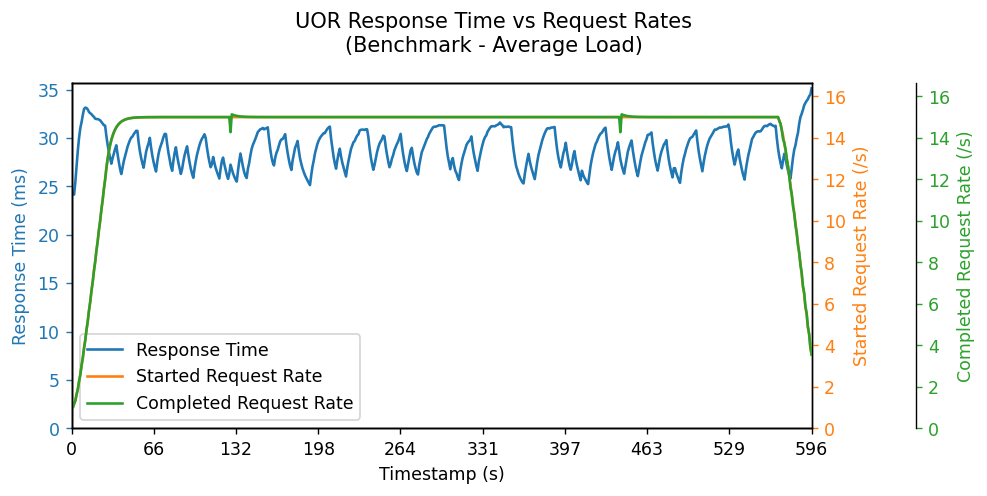
\includegraphics[width=0.8\textwidth]{figures/uor-benchmark-average.png}
    \caption{UOR response time vs. request rate graph - average load benchmark}
    \label{figure:uor-benchmark-average}
\end{figure}

Both response time and request rate degradation can be observed in the local spike test (Fig. \ref{figure:uor-benchmark-spike}). After reaching \textasciitilde40 requests per second, the response time rapidly increases, and the request completion rate starts to diverge from the request start rate. At 45 requests per second (RPS), the response time average increases past 100 milliseconds, and reaches tens of thousands of milliseconds as the request rate continues to increase. During the test, the request start rate is also seen degrading (between 135 and 189 seconds). This is because of the virtual user limit of 2000 set on the k6 test client, which was configured to prevent system resource starvation by the test client. The response time does not appear to recover towards the end of the test. Approximately 0.036\% of requests in the spike tests failed, while neither the average or stress load tests had any failed requests.

\begin{figure}[H]
    \centering
    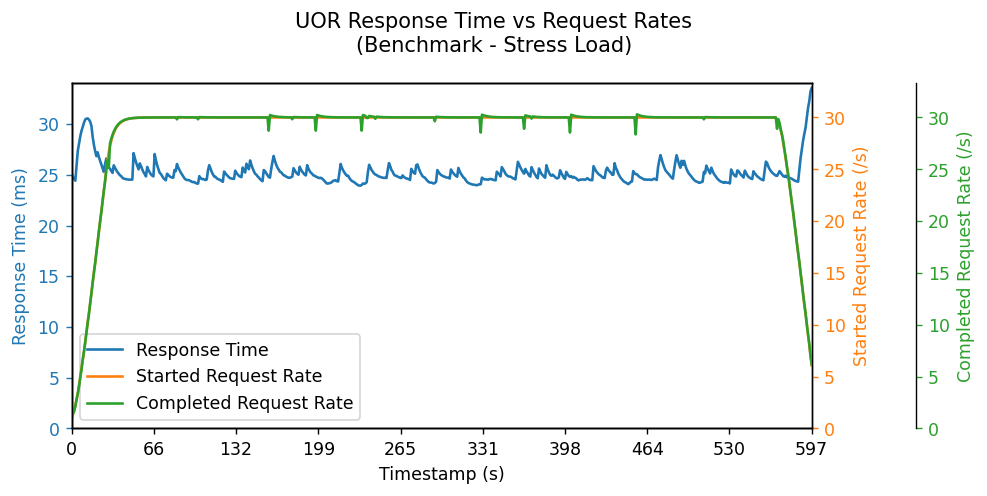
\includegraphics[width=0.8\textwidth]{figures/uor-benchmark-stress.png}
    \caption{UOR response time vs. request rate graph - stress load benchmark}
    \label{figure:uor-benchmark-stress}
\end{figure}

\begin{figure}[H]
    \centering
    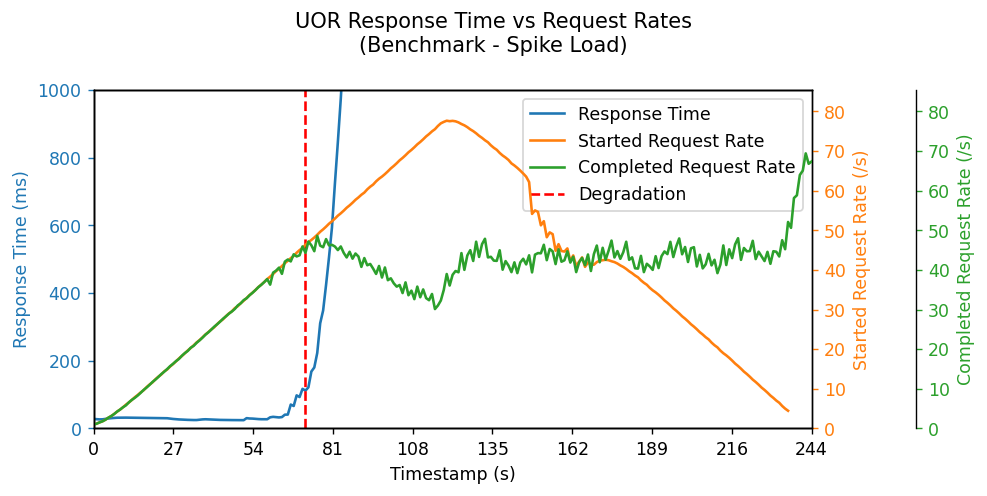
\includegraphics[width=0.8\textwidth]{figures/uor-benchmark-spike.png}
    \caption{UOR response time vs. request rate graph - spike load benchmark}
    \label{figure:uor-benchmark-spike}
\end{figure}

The breakpoint test (Fig. \ref{figure:uor-benchmark-breakpoint}) also identifies this same 45 RPS threshold, beyond which the average response time exceeds 100 milliseconds, and the request completion rate also diverges. No requests failed in the breakpoint tests, but this in part due to the early termination threshold used by breakpoint tests.

\begin{figure}[H]
    \centering
    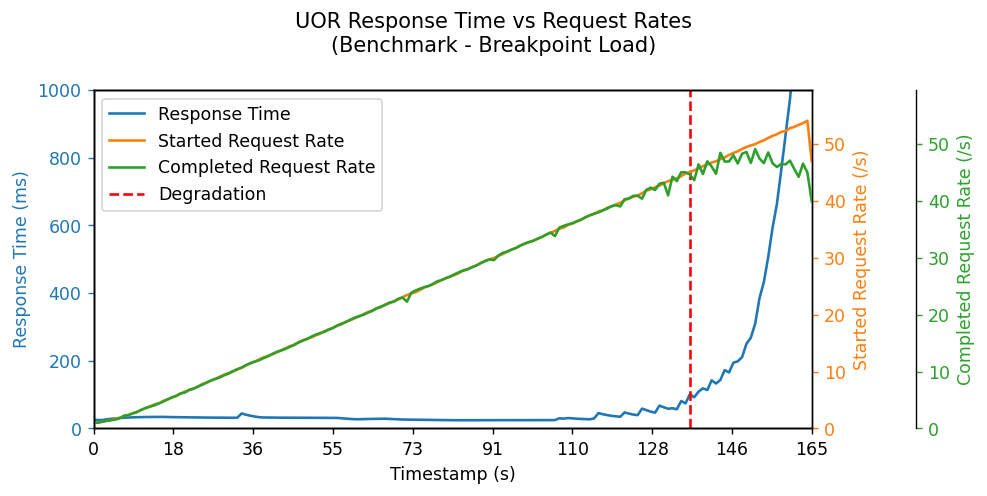
\includegraphics[width=0.8\textwidth]{figures/uor-benchmark-breakpoint.png}
    \caption{UOR response time vs. request rate graph - breakpoint load benchmark}
    \label{figure:uor-benchmark-breakpoint}
\end{figure}



\subsection{Replica count}

\begin{figure}[h]
    \centering
    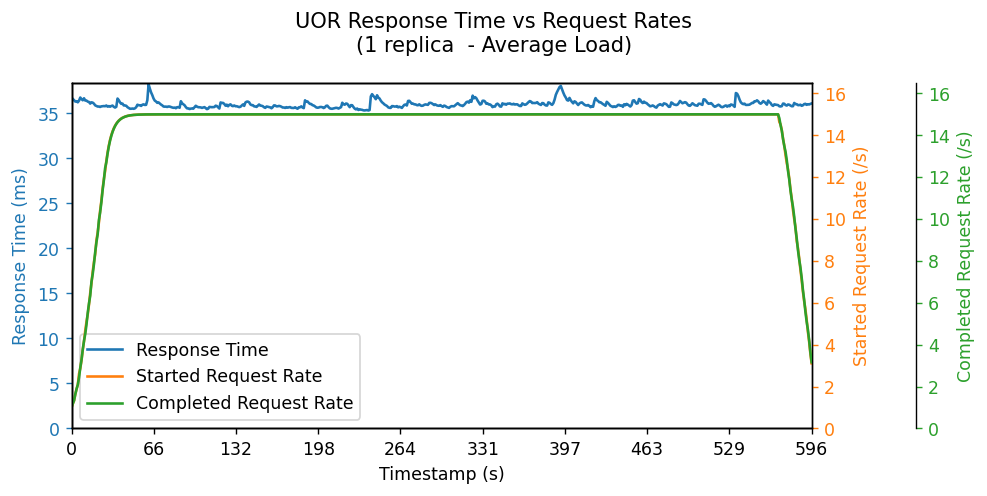
\includegraphics[width=0.8\textwidth]{figures/uor-replica-count-i1-average.png}
    \caption{UOR response time vs. request rate graph - breakpoint load with one replica}
    \label{figure:uor-replica-count-i1-average}
\end{figure}

Using an average load profile against a Django deployment configuration with one replica allows some differences to be observed between the average load benchmark and this cluster-bound test. While the response time of the benchmark sits between 25 and 30 milliseconds, the single replica test sees a median average response time of 35.74 milliseconds (Fig. \ref{figure:uor-replica-count-i1-average}).

\begin{figure}[h]
    \centering
    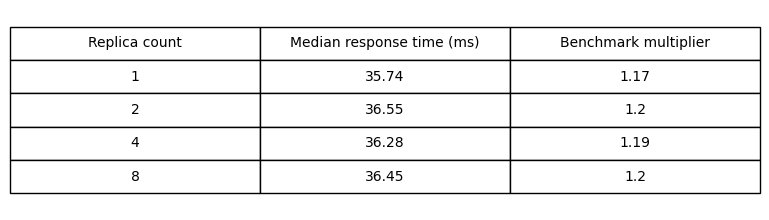
\includegraphics[width=0.8\textwidth]{figures/uor-replica-count-rt-comparison.png}
    \caption{Table of median response times by replica count, average load}
    \label{figure:uor-replica-count-rt-comparison}
\end{figure}

This higher response time average is consistent with any number of replicas (as seen in Fig. \ref{figure:uor-replica-count-rt-comparison}) when average load is applied. The simple explanation for this difference is the use of TLS in the HTTPS connections used between the test client and the cluster, which may take between 5 and 10 milliseconds per request. Unencrypted HTTP is used to access the local deployment, so less work is required to establish a connection. As well as this, the 5 millisecond artificial delay added for cluster-bound requests partially accounts for this discrepancy. A similar range of averages is observed within the replica count stress tests, albeit with a larger gap between the benchmark and replica count median response times (due to the lower average achieved by the benchmark in stress tests compared with the average load tests.)

\begin{figure}[h]
    \centering
    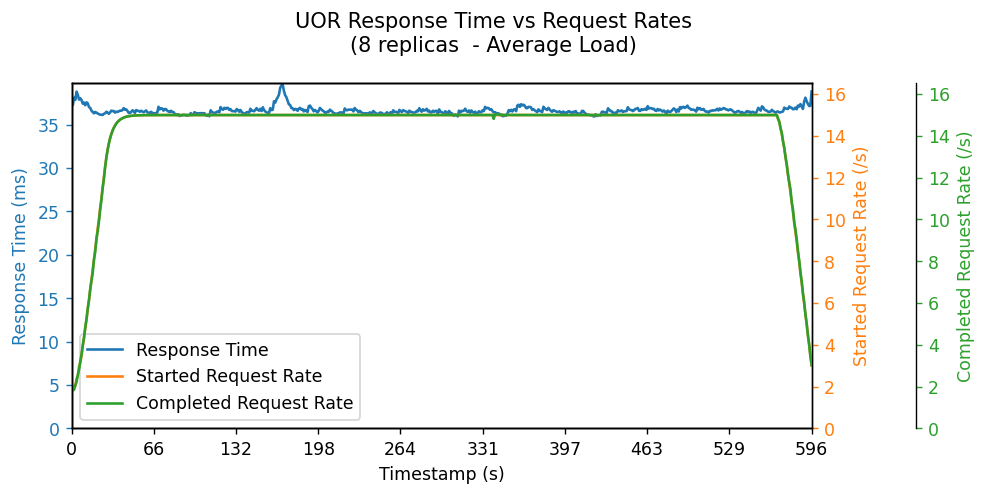
\includegraphics[width=0.8\textwidth]{figures/uor-replica-count-i4-average.png}
    \caption{UOR response time vs. request rate graph - breakpoint load with eight replicas}
    \label{figure:uor-replica-count-i4-average}
\end{figure}

Regardless, any tested number of Django replicas running on the cluster is able to process incoming requests as fast as they arrive (evidenced in Fig \ref{figure:uor-replica-count-i1-average} and \ref{figure:uor-replica-count-i4-average}), so there are no significant request rate differences between the benchmarks and the replica count experiments. However, where the benchmarked local deployment shows evidence of performing worse than the clustered deployment is when testing spike and breakpoint loads with more than one replica. As shown in Fig. \ref{figure:uor-replica-count-rt-comp-spike}, a replica count of one performs similar to the benchmark, where the median response time reaches almost 17,000 milliseconds. The median response times for the remaining replica counts (2, 4 and 6) are far lower, ranging from 39.89 to 42.14 milliseconds.

\begin{figure}[h]
    \centering
    \begin{subfigure}{.5\textwidth}
      \centering
      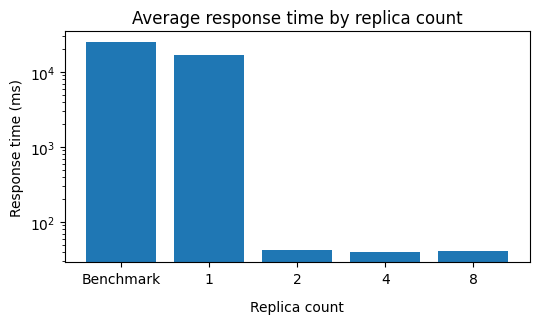
\includegraphics[width=\linewidth]{figures/uor-replica-count-rt-comp-spike1.png}
      \caption{Logarithmic scale}
    \end{subfigure}%
    \begin{subfigure}{.5\textwidth}
      \centering
      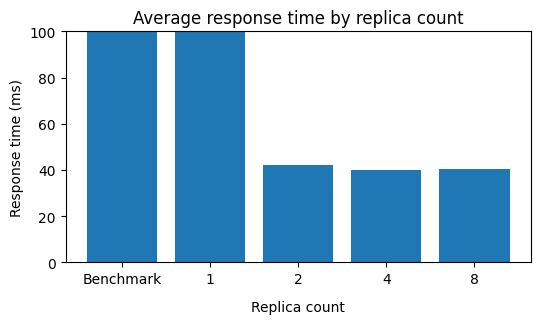
\includegraphics[width=\linewidth]{figures/uor-replica-count-rt-comp-spike2.png}
      \caption{Linear scale}
    \end{subfigure}

    \caption{Median response times by replica count (spike load)}
    \label{figure:uor-replica-count-rt-comp-spike}
\end{figure}

\subsection{Resource allocation and utilisation}


% \subsection{Minimum replicas}
% \subsubsection{Average load}
% \subsubsection{Stress load}
% \subsubsection{Spike load}
% \subsubsection{Breakpoint load}

\section{Flowsheet solving (FS) experiment results}

\subsection{Benchmarks}


\subsection{Replica count}


\subsection{Resource allocation and utilisation}


% \subsection{Minimum replicas}
% \subsubsection{Average load}
% \subsubsection{Stress load}
% \subsubsection{Spike load}
% \subsubsection{Breakpoint load}

\section{Impacts}
Efficiency, accuracy, feasibility (examples of demonstrable impacts).
\section{Threats to validity}

\chapter{Conclusion and Future Work}

\printbibliography

\end{document}
